\chapter{Sexual violence, conflict, and female empowerment}
\chapterauthor{Koen Leuveld}

\label{chap:congogbv}
\renewcommand{\thetable}{\arabic{chapter}.\arabic{table}}


\todo{p.93 en verder (interpretatie resultaten): Ik denk dat je het eerdere punt netjes hebt opgelost ("conflict data over een andere periode dan de SGBV data"). Maar ik heb hier toch een vraagje over. Je zegt dat (historical) conflict kan leiden tot een vervaging van normen, die kunnen leiden tot geweld tegen vrouwen. Dat klinkt redelijk, maar klopt volgens mij niet helemaal met je analyse want normen zeggen (volgens mij) iets over een gemeenschap, maar blootstelling aan geweld en SGNV is een variabele voor individuele vrouwen. Als normen vervagen dan worden zowel vrouwen die wel als niet aan conflict zijn blootgesteld vaker het slachtoffer van misbruik (zou ik denken). Je vindt iets anders, namelijk dat vrouwen die geweld hebben meegemaakt vaker te maken krijgen met SGBV in hun latere leven dan vrouwen die dit niet hebben meegemaakt (misschien hun buren, hebben dus te maken met dezelfde normen). Mijn interpretatie is: door een geschiedenis van geweld wordt een individuele vrouw "minder waard" (damaged goods) en daarom vaker slachtoffer van follow-up geweld. Het interessante resultaat van je multivariate analyse is dat waardevermindering en status in het huishouden allebei een (additief) effect op SGBV lijken te hebben. Het maakt niet uit of je ouders veel land of niet, als jij geweld meemaakt dan gaat je bargaining positie omlaag. Als je ouders weinig land hadden en je hebt zelf geweld meegemaakt, dan heb je dubbel pech. Met andere woorden: het is misschien goed een paar zinnen toe te voegen wat je precies bedoelt met "normen"--op huishoud of gemeenschapsniveau?--en aangeeft hoe dit van invloed kan zijn op SGBV. Ik vind dit trouwens ondanks alle dataproblemen een interessant hoofdstuk.}

\begin{abstract}
The high incidence rate of Sexual and Gender-based Violence in the Democratic Republic of the Congo presents a large human rights problem. Despite the attention this topic has been given, much is unclear about the drivers of SGBV, as accurate data on the subject is difficult to collect. In this paper, I explore the characteristics of the victims SGBV to uncover the dynamics and potential drivers of SGBV. I focus on conflict and female empowerment as potential drivers. In order to avoid social desirability bias and obtain reliable data on this incidence, I conducted a list experiment. I combine the data from this list experiment with rich data on respondents' households, which allows me to separate conflict into recent conflict and historic conflict; and have detailed information on the position of women within their households.

I find that 30\% of the women in my sample have been victimized in the 12 months prior to the interview. The victims are likely to be married to higher-status men, have low intra-household bargaining power, and have been exposed to violent conflict to the extent where they have lost family or household members before 2012 (two years before the list experiment). These findings coincide with the view of a long-lasting impact of conflict on SGBV rates, mainly through Intimate Partner Violence (IPV). This means that human rights abuses  persist long after the end of conflict. Strong measures to structurally improve the position of women in the household and society as a whole are required to address this.
\end{abstract}


%%%%%%%%%%%%%%%%%%%%%%%%%%
\section{Introduction}
%%%%%%%%%%%%%%%%%%%%%%%%%
%Hook
Over the past decades, tremendous progress has been made worldwide to improve the lives of the world's poor. The proportion of people living under the poverty line of \$1.25 per day dropped from over half to just 14\%; gender disparity in primary education has been drastically reduced or even eliminated; under-five mortality rates have been halved \citep{UnitedNations2015}. However, such progress has largely bypassed fragile states, like the Democratic Republic of the Congo (DRC) \citep{Asadullah2018,Samy2011}. Congolese women in particular face economic hardships and human rights violations, including a high rate of Sexual and Gender Based Violence (SGBV): estimates of the proportion of women who have suffered from this range from 15\% to 40\% \citep{Johnson2010,Peterman2011}. Aid workers have called the country ``the world's worst place to be a woman or a child'', and the UN's Special Representative on Sexual Violence in Conflict, Margot Wallstr\"{o}m, even called the country the ``rape capital of the world'' \citep{HumanRightsWatch2009}. The issue of SGBV is of specific concern, given its high psychological, social and economic costs \citep{Post2002,Peterson2018}. Consequently, tremendous international efforts have been made to implement or support projects to assist the victims of SGBV. The 2018 Nobel Peace prize was awarded to Dr. Denis Mukwege, for his work on victims of SGBV at Bukavu's Panzi Hospital.

%add some examples of studies: like tia etc.
Despite this attention, very little reliable data exists on the topic \citep{Palermo2011}. Data collection efforts have been hampered by the conflicts the country has faced, which have made large-scale data collection from representative samples difficult. As a result, most data available on the topic is from surveys within clinics and NGOs aimed at assisting victims of SGBV, making comparison between victims of SGBV and non-victims difficult. These samples are obviously skewed, as they only survey women who have already come forward in search for help. Even when survey data is available, the sensitive nature of the topic may cause respondents to withhold information due their unease in discussing sensitive topics with survey field staff.


%hoort dit bij de vraag?
In this paper, I explore the characteristics of victims of SGBV as well as non-victims to study the dynamics and potential drivers of SGBV. I classify female survey respondents according to potential risk factors for SGBV, and analyse whether these factors are in fact associated with the incidence of SGBV. In this way, this paper aims to address the question what the drivers of SGBV in Eastern Congo are. Specifically, I consider conflict and the position of women in Congolese society as potential drivers, and compare their relative contribution.

The conflict that has persisted in the country for the past decades is the most often-cited driver of the high rate of SGBV.  This is particularly true for policy circles, where the framing of SGBV in Congo as ``weapon of war'' is popular \citep{Baaz2013,Kirby2015}. There is empirical evidence to support this notion. \cite{Johnson2010} carried out a large-scale survey in Eastern Congo to investigate incidence and perpetrators of SGBV, and found that the majority of sexual violence reported by their respondents was conflict-related; of female victims of sexual violence, 74.3\% reported the perpetrators to be conflict-related. Likewise, \citet{Bartels2013} find that the majority of the victims of SGBV treated at Panzi Hospital -- in Bukavu, South Kivu -- indicate that the perpetrators were armed groups. It is therefore not surprising that the topic of SGBV in Congo has often been analysed within the context of violent conflict \citep{Baaz2013}. Conversely, the aspect of the conflict that has received the most world-wide media attention has been SGBV \citep{Autesserre2012a}.  

However, this view of the central role of conflict in sexual violence in the DRC has come under increasing scrutiny. It has been argued that this focus on the relationship between sexual violence and conflict has been counter-productive, as it has distracted attention from other pressing problems the DRC faces \citep{Autesserre2012a, Hilhorst2018,Porter2019}. Moreover, it risks missing the civilian perpetrators of SGBV. There is empirical evidence for this position too. Based on DHS data, \cite{Peterman2011} find that rates of Sexual Intimate Partner Violence (IPV) are higher than rates of other forms of Sexual Violence in Congo. 

This increased focus on IPV, rather than conflict, shifts attention from conflict to the bargaining position of women in Congolese society and households as a driver of SGBV. The bargaining position of a woman is the level of autonomy she has, and is determined by things such as her outside options; its effect on SGBV is ambiguous \citep{Eswaran2011}. One the one hand, a woman's welfare may depend on her bargaining position: women with more income, and better prospects in case of a divorce would thus face less risk of IPV. On the other hand a  woman's partner may use IPV as an instrument to assert power as a response to her increased empowerment. The empirical record reflects this ambiguity. \cite{Bhattacharya} find that increase in employment, and the increasing of status of a woman within the household reduces violence. Similarly, \cite{Hidrobo2016} find that cash transfers to women, decrease the risk of violence. However, when specifically looking at sexual IPV in the Dominican Republic, \cite{Bueno2017} find that an increase in women's (economic) empowerment led to an increase in IPV. In Vietnam, \citep{Bulte2019} find that a project aiming to increase women's income, may have led to increased IPV. In Afghanistan, \cite{Gibbs2020} find no link (positive or negative) between economic empowerment and IPV. The link between IPV and women's intra-household bargaining position may be moderated by local customs, and depend on exactly the type of IPV and the type of empowerment under consideration.

These two main drivers of SGBV -- conflict and empowerment -- are not necessarily separate, as conflict may affect empowerment on the long run. In the short run, conflict may have a direct effect on SGBV through perpetration by armed groups, potentially in a strategic manner \citep{Baaz2013,Kirby2015}. This  caused the topic to be on the international agenda, as a ``weapon of war''. However, in the long run there is a more indirect effect as well: conflict causes the breakdown of norms, which may have long-lasting effects. For example, \cite{Kelly2018} find that that IPV increased in districts that experienced conflict in Liberia, while \cite{Muller2019} draw similar conclusions from data from the Gaza strip. \cite{Saile2013} investigate the correlates of IPV for a sample of conflict-exposed women in Northern Uganda. They find that while the level of conflict exposure predicts physical violence, sexual violence is more associated with the level of childhood familial violence. This link between current and past experiences of violence suggests that the effect of conflict on violence is deeper than just the direct effect. People traumatized during the conflict (either because they were victims or perpetrators) are more likely to be victimized later on. 

In answering the question what the main drivers of SGBV are, I thus consider two main drivers:  the position of women in Congolese society and conflict. Within conflict, I distinguish between historic conflict (here I use pre-2012 data) with long-term, indirect, effects and recent conflict (up to one year prior to the interview) with short-term, direct effects. I argue that the indirect long-term effects of conflict are likely to be related to the position of women, through changing norms, while more recent conflict events may not have had an additional impact on norms yet. For empowerment, I use a bargaining game, and survey questions that determine women's pre-marriage relative status. 

This paper contributes to the empirical evidence base on the incidence of SGBV in Eastern Congo by drawing on a sample of beneficiaries of development assistance projects in South Kivu province, in the Eastern DRC. While the selection of respondents was not done to produce a representative sample for the province, it does not suffer from the same problems that clinic-based surveys have, allowing me to compare victims of SGBV with non-victims. Data on SGBV comes from a list experiment, a technique which has been gaining popularity as a way to obtain information on sensitive topics \citep[see e.g.][]{Sniderman1991,Holbrook2010,Bulte2019,Peterman2018,LaBrie2000,Corstange2009}. Put briefly, list experiments allow group-level analysis of SGBV victimization, without individuals revealing their own victimization status. This eliminates the need for respondents to withhold information and thus reduces the social desirability bias that results \cite{Blair2012}. Such bias may explain the fact that studies on the drivers of SGBV often contradict each other. While one study finds conflict-related perpetrators are responsible for the majority of cases of SGBV \citep{Johnson2010}, another finds intimate partners as the most common culprits \citep{Peterman2011}.\citet{Stark2017} provides an example of how different methodologies can provide different answers: when drawing on Audio Assisted Self-Interviews (ACASI) and find that intimate partners are the main perpetrators of SBV. However, in complementary group discussions, where social desirability bias is likely to be present, respondents did not bring up intimate partners at all. 

I combine list experiments with detailed survey data on the household and outcomes from behavioural experiments, which allows for a rich characterization of victims of SGBV.  Because such a characterization is lacking thus far, this data is useful in addressing and preventing SGBV. Moreover, while the potential drivers of SGBV mentioned above -- conflict and empowerment -- have been studied in isolation, this paper contributes by analysing these in one framework.
%perhaps note that tia finds no predictors for SGBV.

%Road Map
I find high victimization rates in my sample: 30\% of the women report SGBV in the past twelve months. These victims are likely to be married to higher-status men, have low intra-household bargaining power, and have been exposed to violent conflict to the extent where they have lost family or household members before 2012 (two years before the list experiment). I find no evidence of a link between SGBV and recent conflict exposure. These findings are consistent with recent findings in the literature that conflict has long-lasting impact on SGBV through IPV. This paper is structured as follows: first I describe the research setting, the sample, and then the various sources of data. The subsequent section describes my empirical framework, which revolves around the use of a list experiment. I then present the results of the analyses. In the concluding section I contextualize the findings and present policy implications.

%%%%%%%%%%%%%%%%%%%%%%%%%%%%%%%%
\section{Background}
%%%%%%%%%%%%%%%%%%%%%%%%%%%%%%%%
Congo's 2006 constitution grants equal rights to men and women. In practice, however, women hold an inferior position in Congolese society. This is reflected in social and economic outcomes. The literacy rates among women and girls aged 15-24 is 73.6\% (compared to 91.2\% among men and boys of the same age); only 8.5\% of women have completed secondary education (compared to 16.2\% of the men); while 67\% of women work, only 7.8\% work outside of agriculture or trading and services \citep{DHSCongoReport}. Within the household, women occupy an inferior position as well: the husband is the head by law, and marital rape is not considered a crime \citep{Kilonzo2009}. 

In addition to the difficulties inherent to their inferior position, women have faced widespread human rights abuses during the conflicts that have swept the country since the mid 1990s. South Kivu (the setting for the present study) has been greatly affected by these conflicts. The first Congo war started with an invasion by Rwanda and armed groups supported by Rwanda to clear perpetrators of the Rwanda genocide from the refugee camps in the east of the country, putting the province on the front line. Throughout this First Congo War (1996-1997), the Second Congo War (1998-2003) and the subsequent fragile peace, ethnic tensions have remained high throughout the province, resulting in frequent localized bursts of violence \citep[see e.g.][]{Verwijen2016}. While some of the human rights abuses during these phases of the conflict occurred during large-scale attacks on civilians, often they occurred during ambushes while women were conducting their day-to-day tasks \citep{Freedman2011,HRW2002}. Women were often assaulted by multiple perpetrators. These were not only members of rebel groups, but also the government army \citep{HumanRightsWatch2009}. 

The consequences of (conflict-related) SGBV for the victims have been well-researched. It has severe mental and physical health consequences \citep{Johnson2010}. However, due to the remote nature and lack of resources, victims have difficulty finding professional help, often having to travel more than a day to clinics \citep{HarvardHumanitarianInitiative2009,Kohli2012}. The negative consequences persist until long after the event, as victims face stigmatization within their communities and households \citep{Albutt2017,HarvardHumanitarianInitiative2009}.

The adverse consequences of conflict-related SGBV do not remain limited to the direct victims. The violence against women during the conflict resulted in a change in norms, where armed groups were no longer the main perpetrators of SGBV, but civilians (including intimate partners) \citep{Freedman2011}. Risk factors for sexual IPV include partner problematic use of alcohol and partner controlling behaviours \citep{Babalola2014}. While the Congolese government has made attempts to address the situation, such as through the Law on the Suppression of Sexual Violence, implementation of these measures has been marred by the general lack of resources state authority in the country \citep{Steiner2009}.

%%%%%%%%%%%%%%%%%%%%%%%%%%%%%%%%
\section{Sample}
%%%%%%%%%%%%%%%%%%%%%%%%%%%%%%%%
%I am glossing over a complication here: there aren't 73 communities; there are 73 groups. Because some communities supplied two groups (for two interventions) this means there is only 65 communities.

The main source of data for this study is the gender module from a household survey that was undertaken in 2014 as the endline survey for the evaluation of Dutch development aid. This evaluation concerned projects ran by four NGOs in the territories of Kabare, Fizi and Uvira, and the commune of Bagira.\footnote{In the remainder of the paper, I will consider Kabare and Bagira to be one ``territory'', since the selected communities in Kabare and Bagira are located close together, in the peri-urban zone of Bukavu.} The baseline for this evaluation was done in 2012. Half of the respondents were selected from communities that benefited from the projects, the other half were selected from comparable households in non-intervention communities. These projects were about agriculture, women's rights and education. Overall, the beneficiaries of the projects were vulnerable, mostly rural, households. An indicator for being beneficiary to any of these projects is included in the full analysis below. In total data was collected in 73 communities. In each community, baseline data was collected on 15 households in 2012; however, due to attrition, 2014 data is available for an average of 12 households per community, for a total of 889 households. 

\begin{threeparttable}
	\caption{Comparison of DHS and sample data}\label{tab:dhs_compare}
	\centering
	{
\def\sym#1{\ifmmode^{#1}\else\(^{#1}\)\fi}
\begin{tabular}{l*{4}{c}}
\hline\hline
                    &\multicolumn{1}{c}{DHS National}&\multicolumn{1}{c}{DHS South Kivu}&\multicolumn{1}{c}{Full Sample}&\multicolumn{1}{c}{Gender Module}\\
                    &        mean&        mean&        mean&        mean\\
\hline
Age of FR           &       31.83&       31.09&       40.60&       41.09\\
Household has a tin roof&        0.33&        0.60&        0.58&        0.61\\
FR completed primary education&        0.47&        0.29&        0.25&        0.25\\
FR completed secondary education&        0.10&        0.06&        0.02&        0.03\\
\hline\hline
\end{tabular}
}

	\begin{tablenotes}
	\small
	\item FR = Female respondent. DHS = Demographic Health Survey \citep{DHSCongoReport}. For the DHS data, means are provided for household members satisfying the same criteria as FRs from the sample: female heads of household, or female spouses of household heads. 
	\item
	\end{tablenotes}
	
\end{threeparttable}

The sampling procedure outlined here is thus unlikely to have produced a nationally (ore even provincially) representative sample. In Table \ref{tab:dhs_compare}, I present a comparison across selected demographics between the full study sample (column 3), and the representative sample from the DHS Program (columns 1-2). Women in the study sample are older, and less likely to have finished school, than the provincial average in South Kivu.

\begin{table}[htb]
\centering
\caption{Gender module sample make up}
\label{tab:bargsample}
\begin{tabular}{l c c c c c}
\toprule
 & \multicolumn{5}{c}{Male Respondent} \\
Female Respondent&Consented&Refused&Absent&No Husband&Total \\
&No.&No.&No.&No.&No. \\
\hline
Consented&184&3&253&153&593 \\
Refused&0&0&0&1&1 \\
Absent&4&0&0&1&5 \\
No Wife&282&3&2&3&290 \\
Total&470&6&255&158&889 \\
\bottomrule
\end{tabular}
\end{table}

Not all households participated fully in the gender module. Where possible, it was administered to both the head of the household and their spouse, so that there were a Female and a Male Respondent to the interview \footnote{In tables, I refer to Male and Female Respondents as MR and FR respectively.}. In the vast majority of the cases, the husband is considered the head, but it was left open to the respondents to indicate the head. Table \ref{tab:bargsample} displays how the sample is built up. In total, there were 889 respondents to the survey. In 593 households, the Female Respondent (the wife of the household head or the female head) consented to responding to the gender module. In 1 household, the female respondent refused; in 5, the Female Respondent was absent during the interview, and in 290 households the head of the household had no wife, and there was thus no Female Respondent. In 470 households, the Male Respondent (usually the household head) consented to the module, 6 refused, 255 Male Respondents were absent, and in 158 households the head of the household was an unmarried woman, meaning that there was no Male Respondent. In 184 households, both husband and wife responded to the module. Efforts to increase this number, by tracking down absent household heads, were constricted by the limited time field teams had in each community due to the security situation at the time of field work. As a consequence of this, sample sizes between various analyses are different: analyses relying on both partners being present - e.g. for the bargaining game - will have a lower sample size than others.

The selection of respondents to the gender module is unlikely to have been random. In column 4 of Table \ref{tab:dhs_compare} selected demographics for the Female Respondents to the gender module are presented. The respondents are slightly older than the full sample, and considerably older than the provincial average. They are slightly more likely to have completed secondary school than the full sample, but less likely than the provincial average. In Table \ref{tab:sample_selection}, I present results from logit models to find correlations between household characteristics and participation in the gender module. The dependent columns of the columns are whether the wife, the husband and the couple participated in the gender module, respectively. There are some selection effects. Households that own tin roofs, are more likely to have a Female Respondent. In households that own livestock, it was less likely that there was a female respondent to the gender module, and more likely to have male respondent. The final analysis below will include these as controls.

%%%%%%%%%%%%%%%%%%%%%%%%%%%%%%%%
\section{Methods}
%%%%%%%%%%%%%%%%%%%%%%%%%%%%%%%%
This paper combines data from the 2014 and 2012 rounds of the survey, with ACLED data. The gender module from the 2014 survey is the main source of data for this paper. The module was administered separately to Male and Female Respondent (with a small part being administered jointly). It contained (i) a list experiment designed to elicit the incidence of SGBV among Female Respondents; (ii) a risk bargaining game to elicit the relative intra-household bargaining position of the Male and Female Respondent; and (iii) a set of propositions to collect detailed information on gender attitudes. I present the List Experiment, and the analysis thereof, in more detail in the Empirical Framework below. 

\begin{table}[htb]
	\centering
	\caption{Bargaining game lotteries}
	\label{tab:bargaining}
	\begin{tabular}{l c c c c}
	\toprule
	\# & Low & High & Expected & Risk aversion \\
	\hline
	1 & 4,000 CDF & 4,000 CDF & 4,000 CDF & Extremely risk-averse \\
	2 & 3,600 CDF & 4,800 CDF & 4,200 CDF & Extremely risk-averse \\
	3 & 3,200 CDF & 5,600 CDF & 4,400 CDF & Moderately risk-averse \\
	4 & 2,800 CDF & 6,400 CDF & 4,600 CDF & Moderately risk-averse \\
	5 & 2,400 CDF & 7,200 CDF & 4,800 CDF & Risk-neutral \\
	6 & 1,400 CDF & 8,200 CDF & 4,800 CDF & Risk-loving \\ 
	\bottomrule
	\end{tabular}
\end{table}

The risk bargaining game in the gender module was modified from \cite{Martinsson2009}. In the game, the respondents chose between a set of six risky lotteries, based on \cite{Eckel2002}. The lotteries presented ranged from fairly low-risk ones -- where low and high pay-out were nearly equal -- to high-risk one -- where there was a large difference between high and low pay-outs (see Table \ref{tab:bargaining} for details of the lotteries). The Male and Female Respondents first chose privately (without knowing their partner's choice), and then jointly. By comparing the couple decision with the individual decision, I obtain an indicator for bargaining power: the closer the couple decision is to the Female Respondent's decision -- relative to the Male Respondent's decision -- the higher her bargaining power. The difference between the procedure used by \cite{Martinsson2009} and the one here, is that they use a risk experiment based on \cite{Holt2002}; a more complicated experiment compared to \citeauthor{Eckel2002}. This added complication may cause some participants to not fully understand the procedure, leading to poor results \citep{Dave2010a}. Given the low numeracy of the subjects, I implemented the simpler of the two experiments.

I draw on two sources for conflict data: data from the 2012 round of the survey, and ACLED data from 2013-2014. The 2012 data contains detailed information of the conflict history of the respondents dating back to the start of the First Congo War in 1996. Among other things, respondents were asked whether they lost family members, whether they lost property, and when these events took place. I use this to construct indicators for historic victimization, which may have indirect effects on SGBV victimization.  Due to time constraints, the 2014 round of the survey did not contain a detailed conflict exposure module. In order to get more detailed information on recent victimization, complement the household-level data with more recent data from the Armed Conflict Location \& Event Data Project \citep[ACLED;][]{Raleigh2010}. The 2014 data contains GPS coordinates for all interviewed households. Using these coordinates, I can link households to nearby conflict events from the ACLED database that took place within the 12 months preceding the interview. Because this data then coincides with the window for SGBV used here, any direct effects from conflict -- like perpetration of SGBV by armed groups -- will be captured by this indicator. However, while this data is more recent, it does not capture individual experience; only exposure based on the distance from the household to conflict events. 


%%%%%%%%%%%%%%%%%%%%%%%%%%%%%%%%%%%%%%
\section{Empirical Strategy}
%%%%%%%%%%%%%%%%%%%%%%%%%%%%%%%%%%%%%
%what are they?
%A qualitative analysis of disclosure patterns among women with sexual violence-related pregnancies in eastern democratic republic of congo
A major concern in collecting data on SGBV is reporting bias. Respondents are unlikely to be comfortable to truthfully answer questions about SGBV. Respondents may want to hide undesirable answers, leading to what's called social desirability bias. Not only may this lead to an underestimate of the incidence of SGBV, the unwillingness to divulge information may be correlated to the identity of the perpetrators: people may be more willing to divulge victimization from armed groups, than from intimate partners \citep{Stark2017}. This non-random nature of non-response would thus lead to an underestimate of the incidence of SGBV, and biased estimates for the correlates of SGBV when using direct questions. This is why such direct questions are not used in list experiments. Instead, interviewers present respondents with a list of issues and ask them to indicate the number of issues from the list they have faced. By adding the sensitive item to the list of issues for half of the respondents (randomly selected), estimates for incidence of the sensitive item can be obtained by comparing the mean number of issues faced in both groups (hence ``item count technique'' as an alternative name for list experiments). The advantage is thus that answers are guaranteed to be anonymous: the interviewer (or the data analyst) does not know the number of non-sensitive issues the respondent faces and so has no way of knowing the answer to sensitive item. This anonymity removes the need to hide the answer, and thus the social desirability bias. 

%examples:
%\cite{Chuang2019} find that LEs weren't very precise.
%\cite{Peterman2018}
%add some more examples of things that have been studied using LEs.
Over the past decades, list experiments have grown in popularity as a way to obtain accurate data on sensitive topics. \cite{Holbrook2010} review 48 studies using list experiments, and found that they are effective at decreasing social desirability bias. Comparing studies that use list experiments with studies that do not, they find that reporting rates of sensitive items are higher in studies using list experiments. It is therefore not surprising that this approach has been applied to a wide range of topics, such as sensitive political opinions \citep{Frye2017,Blair2014,Meng2017,Corstange2009}, over-reporting of voting \citep{Holbrook2010}, risky behaviours \citep{LaBrie2000} and SGBV \citep{Bulte2019,Peterman2018}.

%hoe ziet mijn implementatie er uit/
For the list experiment in this study, the female respondents were randomly divided into two groups. This was done by the electronic survey software (ODK), based on the randomly assigned ID codes. I follow \cite{Imai2011} in calling these groups Treatment and Control. An interviewer told each respondent: ``I will read 4 \textit{(or 5)} problems that women can experience. These can be sensitive problems. When you've experienced a problem in the last year, please drop one of the balls to the ground. I will not look at when you drop these balls, and only want to know the total number of balls at the end. In the past 12 months, did you experience...
\begin{itemize}
	\item Lack of food;
	\item Lack of money;
	\item Theft;
	\item Sterility; and,
	\item Sexual Violence (Treatment group only)'' %sell dit, mensen kunnen hier moeite mee hebben. Is er een manier om te checken? zeker! check \cite{Chuang2019}!
\end{itemize}

The interviewer only presented women randomly selected to be in the treatment group with the fifth item (Sexual Violence). I selected the four control items in such a way that it is unlikely women in the sample face none, or all, of the issues. In such cases the interviewer knows the respondent's answer to the sensitive issue ("no" if the total number of issues is 0, "yes" if the total number is 5). Not all the control items are non-sensitive, as the item ``sterility'' is a sensitive item. This was done to reduce respondent suspicion when one sensitive items is juxtaposed with a number of completely non-sensitive items (see \citet{Chuang2019} for a more detailed explanation). After all items were read, the interviewer asked the respondent to count the number of balls, and report the number. The questionnaire was field tested prior to field work to ensure that respondents understood these concepts. All interviewers were thoroughly trained in the protocols, and the electronic questionnaire was programmed in such a way to ensure compliance to the protocol.

A crucial assumption for the list experiment is that the randomization ensures that Treatment and Control groups are identical. Table \ref{tab:balance} (Column 7) provides a comparison of the two groups within the sample. The treatment and control group are not perfectly balanced across some of the variables. However, an F-test on the differences between treatment and control being jointly equal to zero fails to reject the null-hypothesis that they are equal (p=0.20). This suggests that the differences found are due to chance, rather than any bias in the randomization procedure.

%hoe doe ik de analyse, en interpreteer ik coefficienten etc.
While the indirect nature of list experiments prevents reporting bias, this does come at a cost of efficiency in statistical analysis. The incidence is easily computed by subtracting the mean of issues faced in the control group from the mean number of issues in the treatment group. This means that sample sizes have to be far larger for list experiments than for direct questions. 

In a regression framework, the incidence would be estimated as follows \citep{Holbrook2010}:

\begin{equation}
\label{eq:basic}
NumIssues_i = \beta_0 + \beta_1 Treatment_i + \epsilon_i
\end{equation}

Where \(NumIssues_i\) is the number of issues experienced by respondent $i$, and \(Treatment_i\) is her treatment assignment. Coefficient \(\beta_1\) yields the estimate for the incidence. To find correlates of SGBV, equation \ref{eq:basic} can be augmented using interaction terms as follows: 
\begin{equation}
\label{eq:congogbv:interaction}
NumIssues_i = \beta_0 + \beta_1 Treatment_i + \beta_2 X_i + \beta_3 Treatment_i X_i + \epsilon_i
\end{equation}

Where \(X_i\) is an explanatory variable and coefficient \(\beta_3\) gives the estimate for the additional incidence of SGBV associated with a unit increase of \(X\). This can be easily modified to allow for more variables. Again, this is much less efficient than when using direct questioning. By using more sophisticated methods proposed by \citet{Imai2011} (and implemented by \cite{Tsai2019} in Stata), more efficient estimates can be obtained. 

\begin{table}[hp] \centering
\newcolumntype{C}{>{\centering\arraybackslash}X}

\caption{Descriptive statistics by treatment assignemt}
\label{tab:balance}
{\footnotesize
\begin{tabularx}{\linewidth}{lCCCCCCC}

\toprule
&{(1)}&{(2)}&{(3)}&{(4)}&{(5)}&{(6)}&{(7)} \tabularnewline
&\multicolumn{2}{c}{All}&\multicolumn{2}{c}{Treatment}&\multicolumn{2}{c}{Control}&{(4)-(6)}\tabularnewline \midrule
{}&{N}&{Mean}&{N}&{Mean}&{N}&{Mean}&{ } \tabularnewline
\midrule \addlinespace[\belowrulesep]
Number of reported issues&593&2.49&291&2.65&302&2.34&0.30*** \tabularnewline
&&(0.94)&&(1.03)&&(0.83)& \tabularnewline
Conflict pre-2012: property lost&530&0.77&264&0.79&266&0.75&0.04 \tabularnewline
&&(0.42)&&(0.41)&&(0.43)& \tabularnewline
Conflict pre-2012: HH member killed&530&0.49&264&0.51&266&0.48&0.03 \tabularnewline
&&(0.50)&&(0.50)&&(0.50)& \tabularnewline
Conflict 2013--2014: Viol. against civilians&496&6.73&239&6.68&257&6.77&--0.08 \tabularnewline
&&(4.69)&&(4.70)&&(4.69)& \tabularnewline
Family MR had more land&450&0.33&224&0.33&226&0.33&--0.00 \tabularnewline
&&(0.47)&&(0.47)&&(0.47)& \tabularnewline
Family FR had more land&450&0.21&224&0.22&226&0.19&0.02 \tabularnewline
&&(0.41)&&(0.41)&&(0.40)& \tabularnewline
Bargaining: choice Female Respondent&593&3.58&291&3.59&302&3.56&0.04 \tabularnewline
&&(2.06)&&(2.08)&&(2.05)& \tabularnewline
Barganing: choice Male Respondent&184&3.45&97&3.49&87&3.40&0.09 \tabularnewline
&&(2.14)&&(2.12)&&(2.18)& \tabularnewline
Bargaining: closer to MR&184&0.40&97&0.37&87&0.44&--0.07 \tabularnewline
&&(0.49)&&(0.49)&&(0.50)& \tabularnewline
Bargaining: closer to FR&184&0.27&97&0.32&87&0.21&0.11* \tabularnewline
&&(0.44)&&(0.47)&&(0.41)& \tabularnewline
Age of FR&593&41.09&291&40.49&302&41.67&--1.17 \tabularnewline
&&(14.01)&&(14.06)&&(13.96)& \tabularnewline
Age of MR&449&45.67&224&44.48&225&46.85&--2.37** \tabularnewline
&&(13.80)&&(13.09)&&(14.40)& \tabularnewline
HH Head Female&593&0.26&291&0.24&302&0.27&--0.03 \tabularnewline
&&(0.44)&&(0.43)&&(0.45)& \tabularnewline
FR completed primary education&593&0.25&291&0.26&302&0.25&0.01 \tabularnewline
&&(0.44)&&(0.44)&&(0.43)& \tabularnewline
FR completed secondary education&593&0.03&291&0.02&302&0.04&--0.02 \tabularnewline
&&(0.17)&&(0.13)&&(0.20)& \tabularnewline
MR completed primary education&449&0.63&224&0.63&225&0.63&0.01 \tabularnewline
&&(0.48)&&(0.48)&&(0.48)& \tabularnewline
MR completed secondary education&449&0.20&224&0.19&225&0.20&--0.01 \tabularnewline
&&(0.40)&&(0.39)&&(0.40)& \tabularnewline
Household has a tin roof&593&0.61&291&0.62&302&0.59&0.03 \tabularnewline
&&(0.49)&&(0.49)&&(0.49)& \tabularnewline
Household owns livestock&593&0.49&291&0.51&302&0.47&0.03 \tabularnewline
&&(0.50)&&(0.50)&&(0.50)& \tabularnewline
territory==Uvira&593&0.24&291&0.24&302&0.23&0.01 \tabularnewline
&&(0.43)&&(0.43)&&(0.42)& \tabularnewline
territory==Fizi&593&0.63&291&0.65&302&0.62&0.03 \tabularnewline
&&(0.48)&&(0.48)&&(0.49)& \tabularnewline
Project Beneficary&593&0.50&291&0.49&302&0.50&--0.01 \tabularnewline
&&(0.50)&&(0.50)&&(0.50)& \tabularnewline
\bottomrule \addlinespace[\belowrulesep]

\end{tabularx}
\begin{flushleft}
\footnotesize FR = Female Respondent; MR = Male Respondent; Standard Deviations in parentheses; *p $<$ 0.1,**p $<$ 0.05,***p $<$ 0.01
\end{flushleft}
}
\end{table}



%%%%%%%%%%%%%%%%%%%%%%%%%%%%%%%%
\section{Results}
%%%%%%%%%%%%%%%%%%%%%%%%%%%%%%%%

\begin{figure}[htb]
  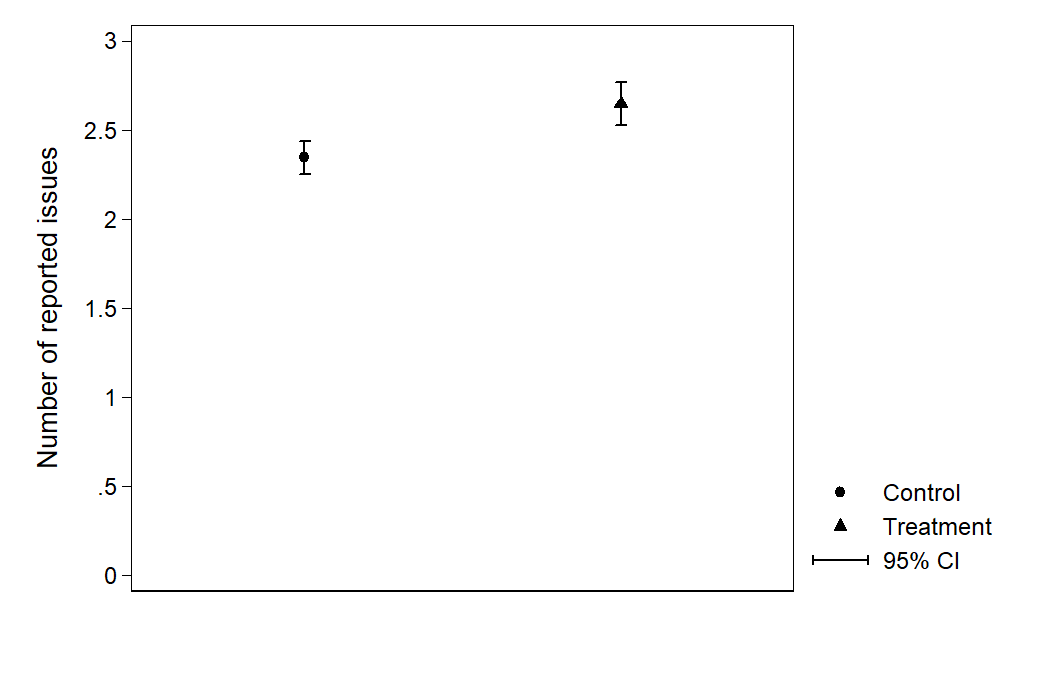
\includegraphics[width=0.6\linewidth]{\congogbvFigures/meancompare_overall.png}
  \caption{Comparison of means of issues faced: treatment vs. control.}
  \label{fig:meancompare_overall}
\end{figure}

In this section, I will first compare the results of the list experiment in the whole sample, then in different sub-groups. I then present results from a full multivariate regression that aims to minimize potential bias caused by confounding variables. 

In the full sample, the difference between the group who were presented with only four issues (the Control group) and the group who were presented four issues plus SGBV (the Treatment group) is the estimate of the incidence of SGBV. The average number of issues reported by the control group is \incid{overall1}{mean0}, while the number if issues reported by the treatment group is \incid{overall1}{mean1} (see Figure \ref{fig:meancompare_overall}). The difference of \incid{overall1}{incidence} implies that the incidence of SGBV is \incid{overall1}{incidence_pct}\% in this sample. The p-value for a t-test on this difference is \incid{overall1}{p}. This estimate appears substantially higher than previous estimates. These previous estimates \citep[e.g.][]{Peterson2018,Stark2017,Johnson2010} arrive at a similar rate of victimization, but over the life of the respondent, whereas here we only consider victimization the past twelve months. A higher incidence is expected, since the sample is non random, drawing mostly from vulnerable rural households. 

\subsection{Conflict} 
%\todo{Erwin 1208: dit is een beetjee onduidelijk. Ik vind het eigenaardig dat je SGBV in 2013-2014 verklaart met conflict in 2011-2012? Misschien moet je het verhaal iets anders opschrijven: (i) we gebruiken de 2012 survey data om iets te zeggen over normen (geweld -> veranderende normen -> SGBV), en (ii) de ACLED data om naar zowel directe en indirecte effecten van geweld te kijken (geweld en SGBV in dezelfde periode). Dit moet denk ik duidelijker worden opgeschreven, en ook worden ingeleid in sectie 1 middels een goede research question.}

\begin{figure}[htb]
  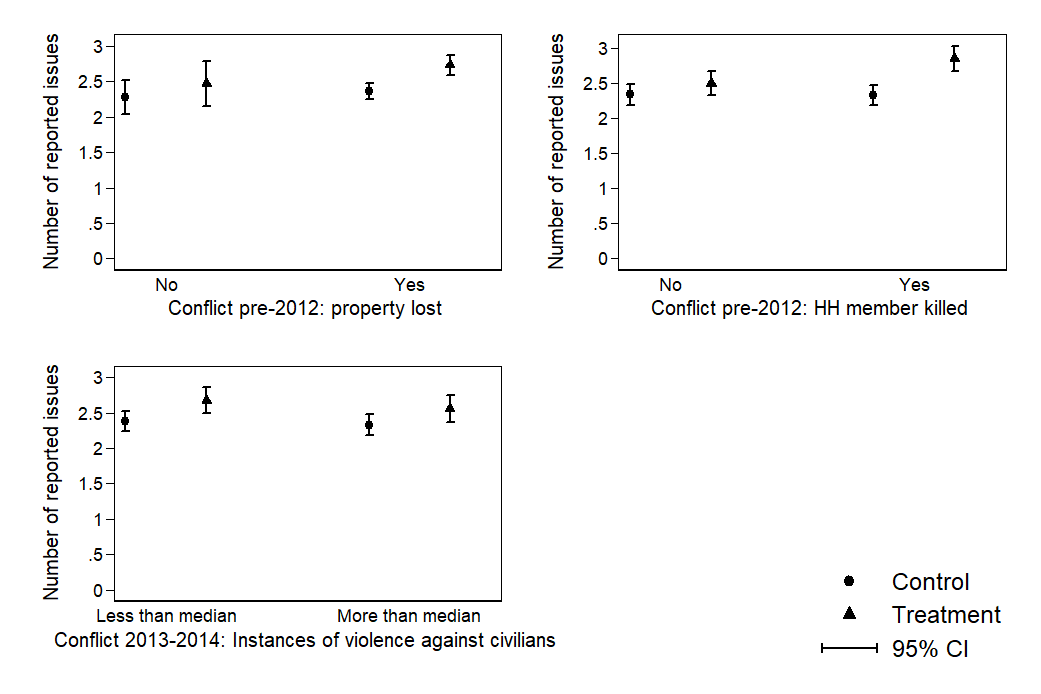
\includegraphics[width=\linewidth]{\congogbvFigures/meancompare_conf.png}
  \caption{Comparison of means of issues faced across conflict exposure.}
  \label{fig:meancompare_conf}
\end{figure}

With respect to conflict, I distinguish between recent conflict (as indicated by ACLED events that happened within the 12 months before the list experiment) and historic conflict (1996-2012). Historic conflict can only have had an indirect effect on SGBV, e.g. through changed norms, as the list experiment only covers SGBV events within the past 12 months. Recent conflict can have a direct effect through perpetration during the conflict event. 

I first analyse victimization patterns by comparing sub-groups of the respondents, based on one variable at a time. A full, multivariate analysis will follow. With respect to conflict, I consider three ways of splitting the sample in sub-groups: (i) respondents who live in households that indicated (or not) in 2012 to have suffered loss of (or damage to) property, including agricultural fields, due to conflict; (ii) whether the respondent's household indicated in 2012 to have lost any household members or family as a consequence of the conflict (or not); and (iii) whether number of instances of violence against civilians in ACLED data within a 10km radius during the past twelve months was higher than the number of instances for the median household (nor not) \footnote{The results presented here are robust to using number of battles or number of fatalities rather than the instances of violence against civilians; using 5,15,20, 25 or 30km as a radius; and using a continuous variable, rather than a binary variable.}. 

Conflict exposure was high in the sample (see Table \ref{tab:balance}): \summstat{victimproplost}{meanall_pct}\% of the respondents reported having lost property due to conflict between 1996 and 2012.  \summstat{victimfamlost}{meanall_pct}\% of the respondents reported the loss of a family or household member. Again, conflict exposure was high, even when limiting the time-span to one year prior to the data collection. The mean number of violent conflicts within a 10km radius was \summstat{acledviolence10}{meanall}. This exposure differs across the territories (Table \ref{tab:conflict_by_terr}). While respondents in all territories were greatly affected by conflict prior to 2012, those in Fizi were hit harder. In the 12 months before the survey however, Uvira was in the midst in an outbreak of violence, related to conflicts surrounding the succession of traditional rulers in the chefferies of Bafuliiro and Plaine de la Ruzizi. In fact, weeks before data collection in 2014 took place, 30 civilians were killed in Mutarule, a village in the Plaine, but not in my sample. This difference in recent and historic conflict patterns means that households with conflict exposure pre-2012 are not more likely to be victimized in 2013-2014 (see also Table \ref{tab:determinants_regression}). Associations between pre-2012 violence and SGBV will thus not be the result of re-targeting of the same households.

\begin{table}[htb]
\centering
\caption{Conflict exposure by territory }
\label{tab:conflict_by_terr}
\input{"\congogbvTables/conflict_by_terr"}
\end{table}

The results of the sub-group analysis is displayed graphically in Figure \ref{fig:meancompare_conf}. From the top two panels, it can be seen that the difference between treatment and control is greater among conflict-victimized respondents than among non-conflict victimized respondents. The size of these differences is listed in Table \ref{tab:meandiff_conf}. Among those that indicated not having lost property, the difference in number of issues faced between treatment and control is 0.19, implying a SGBV victimization rate of 19\%. The difference between Treatment and Control among respondents who did lose property was 0.38. The difference in the differences between these groups of 0.19 issues (this corresponds to coefficient $\beta_3$ in equation \ref{eq:congogbv:interaction} above) is not statistically significant. When splitting the sample by households indicating having lost a family or household member to conflict before 2012, the difference-in-difference estimate is 0.37, indicating that incidence of SGBV among respondents who lost family due to conflict is 37 percentage points higher than among those who have not. This effect is significant at the 5\% level. Note that the SGBV could not have happened during the same time as the conflict event(s): the SGBV happened twelve months before the interview in 2014, while the conflict events happened before 2012.

When looking at more recent exposure to conflict, no clear patterns emerge (see bottom panel of Figure \ref{fig:meancompare_conf}). SGBV incidence among women who have more instances of violence near them than the median is 7 percentage points lower than women who do not (bottom row of Table \ref{tab:meandiff_conf}). However, this is not statistically significant. I thus find no evidence of large-scale direct perpetration of SGBV by armed groups in the one year before data collection, but also no evidence of indirect effects of recent conflict. 

The fact that conflict before 2012 correlates with SGBV, but recent conflict does not, points at a more complex relationship between conflict and SGBV than a simple direct effect due to perpetration by armed groups. It is more likely that violence has an indirect effect through changed norms. The fact that recent conflict seems not to have an indirect effect either, may mean that this change of norms takes time, or that the nature of recent conflict is different from historic conflict. 

%meandifftab is defined in congogbv_customfunctions
\begin{table}[htb]
\caption{Differences in numbers of issued faced in the list experiment, across conflict indicators}
\label{tab:meandiff_conf}
\meandifftab{"\congogbvTables/meandifftab_conf.csv"}
\end{table}

\subsection{Intra-household bargaining position}
\begin{figure}[htb]
  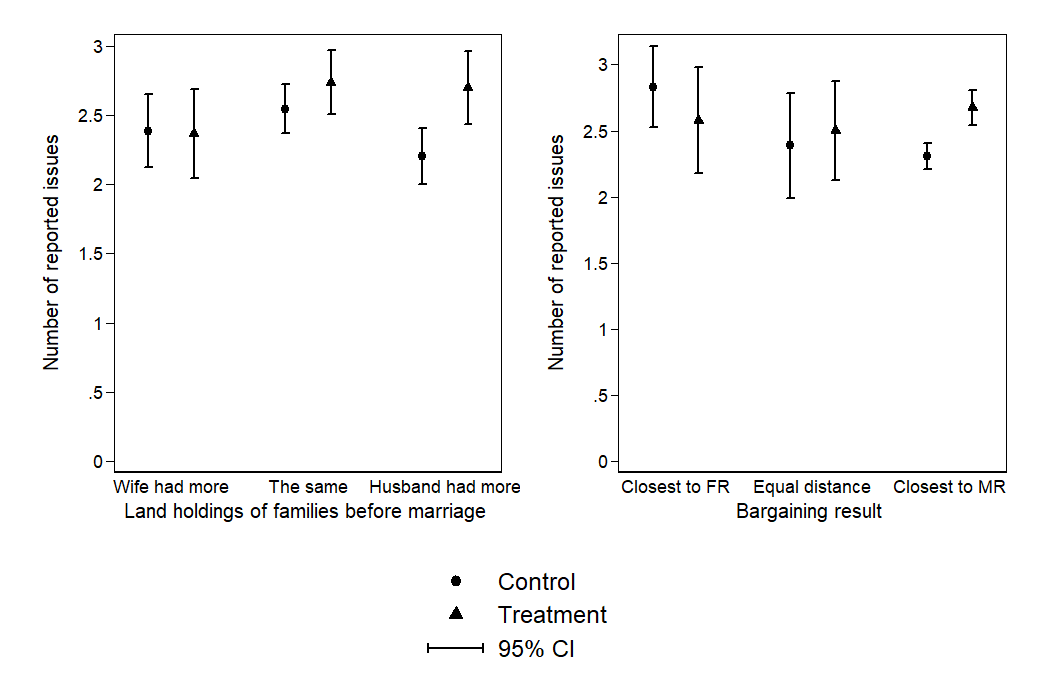
\includegraphics[width=\linewidth]{\congogbvFigures/meancompare_mar.png}
  \caption{Comparison of means of issues faced by pre-marriage status.}
  \label{fig:meancompare_mar}
\end{figure}

I then create sub-groups based on the intra-household bargaining position of the respondents. I compare women across two variables. First, I compare women across the relative status of the partners at the time of marriage, by using family land-holdings as a proxy for status. The 2014 survey contained a section on the marriage of the (spouse of the) household head. In this section, respondents were asked whose family owned more land, prior to the marriage: the wife's, the husband's, or whether they had equal land. This choice of proxy was made in consultation with local partners (including NGOs and universities), and based on the importance of agriculture in the area. In \summstat{husbmoreland}{meanall_pct}\% of the cases, the husband's family had more land, in \summstat{wifemoreland}{meanall_pct}\% of the cases the wife's family did. Note that only \summstat{wifemoreland}{nall} households responded to this question, as some refused to give a definite answer (Table \ref{tab:balance}). 

The second intra-household aspect I explore is derived from the results of the bargaining game played with couples during the 2014 survey. I create three groups, based on whether the joint decision is closer to the husband's decision, to the wife's, or if the distance is equal. The mean choice of the Female Respondents in the sample was \summstat{riskwife}{meanall}; the Male Respondents were slightly more risk-averse: their mean choice was \summstat{riskhusband}{meanall}. In \summstat{barghusbandcloser}{meanall_pct}\% of the cases, the couple decision was closest to the Male Respondent's choice. In \summstat{bargwifecloser}{meanall_pct}\% it was closer to the Female Respondent's. Note that the size of the sample here is smaller than for the other variables presented, as it was not always possible to have both the Male and Female Respondent present at the same time for the interview.

Figure \ref{fig:meancompare_mar} displays the results from the sub-group analysis. Overall, the difference between treatment and control is larger for the sub-groups of respondents with a worse intra-household bargaining position, indicating that the incidence of SGBV is higher among these respondents. As suggested by the large size of the 95\% confidence intervals, some of these sub-groups are small. In Table \ref{tab:meadifftab_mar}, these differences are tabulated, including the sizes of the sub-groups. However, the variable definitions are slightly different, due to the difficulties in interpreting difference-in-differences between three sub-groups. For each variable, two comparisons are tabulated: one, comparing households where the female respondents had the better bargaining position with the two other sub-groups, and one comparing households where the male respondent had the better bargaining position with the two other sub-groups. Female respondent in households where the family of the husband had the most land prior to marriage were victims of SGBV in 50\% of the cases, while 16\% of the other respondents were. The difference of 33 percentage points is statistically significant at the 10\% level. In the other comparison for the same variable, the difference is even larger, but not statistically significant; perhaps due to the low number of women with more pre-marital status than their husbands. The differences when split by results from the bargaining game are larger still: 57 or 61 percentage points, depending on the groups used.

While these results may suggest that IPV is an important driver of SGBV, the fact that I have no information on perpetrators means that this is not certain.


\begin{table}[htb]
\caption{Differences in numbers of issued faced in the list experiment, across intra-household status}
\label{tab:meadifftab_mar}
\meandifftab{"\congogbvTables/meandifftab_mar.csv"}
\end{table}


%%%%%%%%%%%%%%%%%%%%%%%%%%%%%%
\subsection{Multivariate Regression analysis}
%%%%%%%%%%%%%%%%%%%%%%%%%%%%%%

In the preceding sections, I examined univariate relations between variables of interest and the incidence of SGBV. However, such analysis may suffer from omitted variables and spurious correlations. Here I move to a richer specification, in order to prevent such biases, and assess the relative importance of each driver. I expand equation \ref{eq:congogbv:interaction} to simultaneously include indicators for conflict and intra-household bargaining position. To reduce the risk of multi-collinearity, I do not include the full set of variables discussed above, but select one indicator for each, guided by the results obtained above. A key criterion for selection is the number of respondents for each indicator. The analysis of list experiments suffers from rapid loss of power due to the indirect nature of the analysis. To mitigate this, indicators that are available for large groups of respondents were selected. For conflict, I include both the indicator for household member killed before 2012 (as an indicator for historic conflict) and violence against civilians from the ACLED data (as an indicator for recent conflict); and for intra-household bargaining position a dummy for the husband's family having the most land. I use the KICT Stata package developed by \citet{Tsai2019} to estimate these models. Interpretation of the coefficients is the same as equation \ref{eq:congogbv:interaction}, but estimation is more efficient.

In order to reduce missing variable bias, I include a set of controls that likely (co-) determine SGBV and the right-hand side variables listed above. A full analysis of these determinants is provided in the Appendix, Table \ref{tab:determinants_regression}. In addition, I include variables that determine sample selection, as displayed in Table \ref{tab:sample_selection}. In particular, I include the age of the Female Respondent; indicators for the education of the Male and Female respondents; asset holdings of the household, including livestock and a tin roof; territory dummies; and an indicator for being in the treatment group of any of the projects under evaluation for the survey.

In Table \ref{tab:results_regression} I display the results of these regressions. In columns 1-3 I rerun the univariate models from above. Results are the same as before: both conflict history and intra-household bargaining are associated with increased incidence of SGBV. I In column 4 I present the full model. I find that women in a marriage where their husband's family had more land before the marriage, are \coeffget{l5}{Delta:husbmoreland}{coef_pct} percentage points more likely than other women to be victim of SGBV. Note that the pre-marriage status of women within the household is uncorrelated to conflict (see Table \ref{tab:determinants_regression}). Women who live in households that lost a family or household member due to conflict prior to 2012 are \coeffget{l5}{Delta:victimfamlost}{coef_pct} percentage points more likely to be victimized by SGBV than other women. Of note is also the negative associated of the Female Respondent having a secondary education: in this linear model, women with secondary education are \coeffget{l5}{Delta:eduwife_sec}{coef_pct} percentage points less likely to be victimized. The fact that the absolute value of this coefficient is higher than 1 is due to the fact that linear models do not constrain predictions of probabilities between 0 and 1.

The finding that conflict history is associated with an increase in SGBV, while recent conflict is not, points to the indirect relationship between conflict and SGBV, where conflict may affect SGBV rates not through perpetration by armed groups, but by an increase in IPV. The notion that IPV is a major driver of SGBV is reinforced by the fact that both intra-household bargaining position and secondary education are negatively associated with SGBV.  This suggests that the position of women is important in protecting them from human rights violations.

Caution should be taken with this interpretation, as results presented here are not necessarily causal: women with higher education may differ from other women in non-observable ways, and face lower victimization because of that, rather than education. Furthermore, no data exists on the perpetrators of the violence. The method of a list experiment does not allow for follow-up questions to victimized women, as the interviewer cannot know who to ask these follow up questions to.

\begin{threeparttable}
	\caption{Multivariate regression Results}\label{tab:results_regression}
	\centering
	\scriptsize
	{
\def\sym#1{\ifmmode^{#1}\else\(^{#1}\)\fi}
\begin{tabular}{l*{4}{c}}
\hline\hline
                    &\multicolumn{1}{c}{(1)}   &\multicolumn{1}{c}{(2)}   &\multicolumn{1}{c}{(3)}   &\multicolumn{1}{c}{(4)}   \\
\hline
Delta               &               &               &               &               \\
Family MR had more land&       0.419** &               &               &       0.451*  \\
                    &     (0.204)   &               &               &     (0.240)   \\
[1em]
Conflict pre-2012: HH member killed&               &       0.409** &               &       0.374** \\
                    &               &     (0.182)   &               &     (0.179)   \\
[1em]
Conflict 2013-2014: Viol. against civilians&               &               &      0.0120   &      0.0147   \\
                    &               &               &    (0.0224)   &    (0.0230)   \\
[1em]
FR empowerment attitudes&               &               &               &    0.000101   \\
                    &               &               &               &    (0.0199)   \\
[1em]
Age of FR           &     0.00843   &     0.00684   &     0.00563   &      0.0110   \\
                    &    (0.0161)   &    (0.0182)   &    (0.0186)   &    (0.0207)   \\
[1em]
Age of MR           &     -0.0122   &    -0.00929   &    -0.00778   &     -0.0111   \\
                    &    (0.0149)   &    (0.0162)   &    (0.0174)   &    (0.0189)   \\
[1em]
HH Head Female      &     0.00951   &     -0.0766   &       0.257   &       0.421   \\
                    &     (0.445)   &     (0.525)   &     (0.318)   &     (0.410)   \\
[1em]
FR completed secondary education&      -1.111***&      -1.347***&      -1.034***&      -1.249***\\
                    &     (0.320)   &     (0.351)   &     (0.336)   &     (0.332)   \\
[1em]
MR completed primary education&     -0.0390   &     -0.0655   &      -0.193   &      -0.263   \\
                    &     (0.166)   &     (0.178)   &     (0.181)   &     (0.177)   \\
[1em]
Household has a tin roof&       0.292   &       0.279   &       0.184   &       0.214   \\
                    &     (0.203)   &     (0.221)   &     (0.234)   &     (0.233)   \\
[1em]
Household owns livestock&     -0.0455   &    -0.00342   &      -0.142   &      -0.193   \\
                    &     (0.160)   &     (0.181)   &     (0.177)   &     (0.186)   \\
[1em]
territory==Uvira    &       0.418   &       0.202   &       0.438   &       0.205   \\
                    &     (0.264)   &     (0.342)   &     (0.288)   &     (0.360)   \\
[1em]
territory==Fizi     &       0.511*  &       0.232   &       0.504*  &       0.191   \\
                    &     (0.292)   &     (0.365)   &     (0.302)   &     (0.379)   \\
[1em]
Project Beneficary  &      0.0542   &      0.0121   &      0.0382   &      0.0732   \\
                    &     (0.163)   &     (0.177)   &     (0.157)   &     (0.167)   \\
[1em]
Constant            &      -0.162   &    -0.00267   &    -0.00290   &      -0.111   \\
                    &     (0.483)   &     (0.506)   &     (0.491)   &     (0.614)   \\
\hline
Observations        &         449   &         402   &         379   &         350   \\
\hline\hline
\end{tabular}
}

	
	\begin{tablenotes}
	\small
	 \item FR = Male Respondent; MR = Female Respondent
	 \item Standard errors clustered at the village level; * p $<$ 0.1, **, p $<$ 0.05, *** p $<$ 0.01
	\end{tablenotes}

\end{threeparttable}

\section{Conclusion}
%restate the topic and its importance.
In this paper, I analysed the results from a list experiment, in order to identify potential drivers of SGBV in Eastern Congo. Prevalence of SGBV is high in Congo, however little is known about the victims, and the drivers of victimization. In order to address this, I combined the results from the list experiment with rich  data, including a household survey, a bargaining game, and conflict data.

The incidence rates I find are very high: 30\% of the women in the sample report having been the victim of SGBV in the past twelve months. Most data collected on lifetime victimization arrives at similar rates, suggesting that this estimate for a one-year window is high. The rate found here may thus not be nationally, or regionally, representative. This is likely due to the fact that women in the sample were recruited among beneficiaries and potential beneficiaries of programs aimed at assisting the most vulnerable women and households. It is to be expected that incidence rates in this group are higher than for other groups. In fact, I find that secondary schooling rates among women in my sample is lower than the national or provincial average, and that incidence of SGBV among women who have attended secondary school are significantly lower than among other women.

When examining the backgrounds of the victims, I find that they are likely to be married to higher-status men, have low intra-household bargaining power, and have been exposed to violent conflict to the extent where they have lost family or household members before 2012 (two years before the list experiment). When comparing these effects in one analysis, I find that the effect of intra-household dynamics is larger than the effect of conflict. This contrasts with popular frames where the conflict is seen as the primary driver of SGBV, but is in line with previous literature suggesting that intimate partners are more likely perpetrators of SGBV than members of armed groups \citep[see e.g.][]{Peterman2011}.

Taken together, these finding imply that human rights violations do not end when the conflict ends. The disruption of social norms may cause women (and perhaps men, but the present data set does not cover them) to suffer from violence long after the last shot has been fired. A focus of rape as a ``weapon of war'' may thus be too narrow to address these violations. This is not to say there direct perpetration of SGBV by armed forces is not a problem in Congo. There is ample proof that large-scale violations have been committed by armed forces, especially historically. The conflict has undergone changes throughout the years, and with it the kinds of human rights violations perpetrated. The massacre in Mutarule in the weeks before data collections did see 30 innocent civilians murdered, but there are no reports of rape. Furthermore, focusing efforts to assist women on the victims from such attacks risks missing women victimized in their homes, far away from any fighting. Structural changes encouraging women's education and tangibly raising their status are needed to protect these women as well. 

%Unfortunately, often women are less empowered due to intervenstions aimed at protection them \citep{Bashwira2014}.
There are three large caveats with these findings: (i) causal interpretation is difficult due to the cross-sectional nature of the data; (ii) little analysis could be done on the perpetrators of the violence, as indirect questioning precludes probing into this. More research is needed to  to address these important issues; and (iii) I did not  collect data on the victimization of men. More research is needed to address these.

\section{Appendix}
\setcounter{table}{0}
\renewcommand{\thetable}{\arabic{chapter}.A\arabic{table}}
\begin{threeparttable}[htb]
	\scriptsize
	\caption{Sample selection for the Gender Module}\label{tab:sample_selection}
	\begin{center}
	{
\def\sym#1{\ifmmode^{#1}\else\(^{#1}\)\fi}
\begin{tabular}{l*{3}{c}}
\hline\hline
                    &\multicolumn{1}{c}{(1)}   &\multicolumn{1}{c}{(2)}   &\multicolumn{1}{c}{(3)}   \\
                    &        Wife   &     Husband   &      Couple   \\
\hline
                    &               &               &               \\
Age of FR           &     -0.0305** &      0.0244** &     -0.0124   \\
                    &    (0.0126)   &    (0.0112)   &    (0.0127)   \\
[1em]
Age of MR           &      0.0199*  &    -0.00864   &      0.0176   \\
                    &    (0.0118)   &    (0.0110)   &    (0.0130)   \\
[1em]
HH Head Female      &       0.171   &      -1.142*  &           0   \\
                    &     (0.689)   &     (0.602)   &         (.)   \\
[1em]
FR completed primary education&       0.120   &      -0.197   &      -0.109   \\
                    &     (0.224)   &     (0.245)   &     (0.210)   \\
[1em]
FR completed secondary education&       0.484   &      -0.285   &       0.169   \\
                    &     (0.587)   &     (0.399)   &     (0.488)   \\
[1em]
MR completed primary education&     -0.0233   &       0.226   &       0.279   \\
                    &     (0.189)   &     (0.218)   &     (0.230)   \\
[1em]
MR completed secondary education&       0.228   &      -0.208   &    -0.00740   \\
                    &     (0.213)   &     (0.215)   &     (0.212)   \\
[1em]
Household has a tin roof&       0.307*  &      0.0468   &       0.446** \\
                    &     (0.181)   &     (0.171)   &     (0.207)   \\
[1em]
Household owns livestock&      -0.564***&       0.695***&       0.146   \\
                    &     (0.204)   &     (0.189)   &     (0.172)   \\
[1em]
territory==Uvira    &      -0.215   &       1.165***&       0.949***\\
                    &     (0.297)   &     (0.261)   &     (0.336)   \\
[1em]
territory==Fizi     &     -0.0496   &       0.312   &       0.258   \\
                    &     (0.263)   &     (0.217)   &     (0.296)   \\
[1em]
Project Beneficary  &       0.490** &      -0.450** &      0.0594   \\
                    &     (0.195)   &     (0.182)   &     (0.249)   \\
[1em]
Constant            &       0.726*  &      -0.700   &      -2.347***\\
                    &     (0.430)   &     (0.434)   &     (0.429)   \\
\hline
Observations        &         717   &         717   &         704   \\
\hline\hline
\end{tabular}
}

	\begin{tablenotes}
	 \item Standard errors clustered at the village level
	 \item * p $<$ 0.1, **, p $<$ 0.05, *** p $<$ 0.01
	\end{tablenotes}
	\end{center}
\end{threeparttable}

\clearpage

%\begin{landscape}

%note: specialcell is defined in the customfunctions.tex file
\begin{threeparttable}
	\caption{Determinants of Violence and Bargaining Power}\label{tab:determinants_regression}
	\scriptsize 
	\centering
	{
\def\sym#1{\ifmmode^{#1}\else\(^{#1}\)\fi}
\begin{tabular}{l*{3}{c}}
\hline\hline
                    &\multicolumn{1}{c}{(1)}&\multicolumn{1}{c}{(2)}&\multicolumn{1}{c}{(3)}\\
                    &\multicolumn{1}{c}{\specialcell{Family MR\\had more land}}&\multicolumn{1}{c}{\specialcell{Bargaining:\\closer to FR}}&\multicolumn{1}{c}{\specialcell{Conflict pre-2012:\\HH member killed}}\\
\hline
Family MR had more land&               &      0.0756   &       0.679   \\
                    &               &    (0.0554)   &     (0.476)   \\
[1em]
Conflict pre-2012: HH member killed&      0.0799   &               &      -1.494***\\
                    &    (0.0588)   &               &     (0.476)   \\
[1em]
Conflict 2013-2014: Viol. against civilians&     0.00885   &     -0.0184***&               \\
                    &   (0.00627)   &   (0.00477)   &               \\
[1em]
Age of FR           &    -0.00431   &     0.00219   &     -0.0264   \\
                    &   (0.00602)   &   (0.00448)   &    (0.0349)   \\
[1em]
Age of MR           &     0.00355   &    -0.00146   &      0.0281   \\
                    &   (0.00435)   &   (0.00390)   &    (0.0320)   \\
[1em]
FR completed primary education&      0.0542   &      -0.109   &     -0.0536   \\
                    &    (0.0695)   &    (0.0656)   &     (0.672)   \\
[1em]
FR completed secondary education&     -0.0147   &       0.474***&       0.602   \\
                    &     (0.129)   &     (0.147)   &     (1.417)   \\
[1em]
MR completed primary education&      0.0834   &      0.0314   &      -0.347   \\
                    &    (0.0612)   &    (0.0622)   &     (0.512)   \\
[1em]
MR completed secondary education&     -0.0523   &      0.0408   &       0.239   \\
                    &    (0.0703)   &    (0.0764)   &     (0.603)   \\
[1em]
Household has a tin roof&     -0.0267   &      -0.114** &       0.563   \\
                    &    (0.0537)   &    (0.0509)   &     (0.539)   \\
[1em]
Household owns livestock&       0.114** &      0.0536   &      -0.235   \\
                    &    (0.0554)   &    (0.0526)   &     (0.490)   \\
[1em]
territory==Uvira    &     -0.0556   &       0.295***&       3.566***\\
                    &    (0.0589)   &    (0.0904)   &     (1.104)   \\
[1em]
territory==Fizi     &     -0.0166   &       0.404***&      -1.069   \\
                    &    (0.0560)   &    (0.0763)   &     (1.487)   \\
[1em]
Project Beneficary  &     -0.0854*  &      0.0492   &       0.198   \\
                    &    (0.0461)   &    (0.0450)   &     (1.136)   \\
[1em]
Constant            &       0.212   &       0.247** &       6.599***\\
                    &     (0.133)   &     (0.106)   &     (1.420)   \\
\hline
Observations        &         350   &         350   &         350   \\
\hline\hline
\end{tabular}
}

	
	\begin{tablenotes}
	\tiny
	 \item Standard errors clustered at the village level
	 \item * p $<$ 0.1, **, p $<$ 0.05, *** p $<$ 0.01
	\end{tablenotes}
\end{threeparttable}
%\end{landscape}

%bibliography, this is needed for bibtex
\bibliographystyle{chicago}
%path to .bib file (e.g. automatically exported by mendeley) dot not include the file extension!
\bibliography{\bibtex/Thesis-CongoGBV}



